\chapter{System Design}

\section{Chapter Introduction}
In this section I will discuss the architecture of the application. I will discuss the components of an android application mainly Android Activities and the tops that come with Activities; Fragments, Activity lifecycle, persistence, process lifecycle etc. I will also discuss how the Front-End communicates with the Back-End after explaining of activities work.

\section{Introduction to System}
This application was made using Kotlin with Android Studio. My application uses Single Activity App Architecture, which is recommended by Google as the best way to make a Native Android Application\cite{android_single_activity_blog}

\section{Android Activities}
An activity is a single, focused thing that the user can do. Almost all activities interact with the user, so the Activity class takes care of creating a window for you in which you can place your UI with setContentView. While activities are often presented to the user as full-screen windows, they can also be used in other ways: as floating windows (via a theme with android.R.attr\#windowIsFloating set), Multi-Window mode or embedded into other windows.\cite{android_activity_docs} There are two methods almost all subclasses of Activity will implement: 

\begin{itemize}
    \item onCreate  is where you initialize your activity. Most importantly, here you will usually call setContentView(int) with a layout resource defining your UI, and using findViewById to retrieve the widgets in that UI that you need to interact with programmatically.
    \item onPause is where you deal with the user pausing active interaction with the activity. Any changes made by the user should at this point be committed (usually to the android.content.ContentProvider holding the data). In this state the activity is still visible on screen.
\end{itemize}

To be of use with Context.startActivity(), all activity classes must have a corresponding <activity> declaration in their package's \textbf{AndroidManifest.xml.}

\subsection{Fragments}
A Fragment represents a behavior or a portion of user interface in a FragmentActivity. You can combine multiple fragments in a single activity to build a multi-pane UI and reuse a fragment in multiple activities. You can think of a fragment as a modular section of an activity, which has its own lifecycle, receives its own input events, and which you can add or remove while the activity is running (sort of like a "sub activity" that you can reuse in different activities).\cite{android_activity_fragments}\newline

A fragment must always be hosted in an activity and the fragment's lifecycle is directly affected by the host activity's lifecycle. For example, when the activity is paused, so are all fragments in it, and when the activity is destroyed, so are all fragments. However, while an activity is running, you can manipulate each fragment independently, such as add or remove them. When you perform such a fragment transaction, you can also add it to a back stack that's managed by the activity—each back stack entry in the activity is a record of the fragment transaction that occurred. The back stack allows the user to reverse a fragment transaction (navigate backwards), by pressing the Back button.\cite{android_activity_fragments}\newline

When you add a fragment as a part of your activity layout, it lives in a ViewGroup inside the activity's view hierarchy and the fragment defines its own view layout. You can insert a fragment into your activity layout by declaring the fragment in the activity's layout file, as a <fragment> element, or from your application code by adding it to an existing ViewGroup.\cite{android_activity_fragments}\newline

\newpage
\begin{figure}[h!]
	\caption{Android app which uses Architecture components \cite{android_guide_arc}}
	\label{image:myImageName}
	\centering
	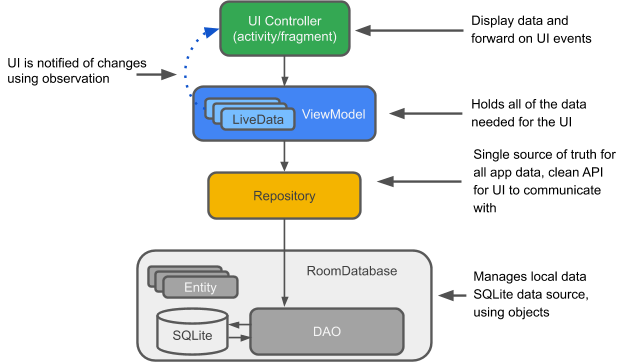
\includegraphics[width=1\textwidth]{Images/android_app_arc.png}
\end{figure}	

\subsection{Creating a Fragment}

Example of Fragment in Project to create the Navigation Bars:\newline

\textbf{HomeViewModel}
\begin{minted}{kotlin}
class HomeViewModel : ViewModel() {

    private val _text = MutableLiveData<String>().apply {
        value = "This is home Fragment"
    }
    val text: LiveData<String> = _text
}
\end{minted}


\textbf{HomeFragment}
\begin{minted}{kotlin}
class HomeFragment : Fragment() {

    private lateinit var homeViewModel: HomeViewModel

    override fun onCreateView(
        inflater: LayoutInflater,
        container: ViewGroup?,
        savedInstanceState: Bundle?
    ): View? {
        homeViewModel =
            ViewModelProviders.of(this).get(HomeViewModel::class.java)
        val root = inflater.inflate(R.layout.fragment_home, container, false)
        val textView: TextView = root.findViewById(R.id.text_home)
        homeViewModel.text.observe(this, Observer {
            textView.text = it
        })
        return root
    }
}
\end{minted}

After creating a fragment you then need to declare it inside an activity layout file
\begin{minted}{kotlin}
<?xml version="1.0" encoding="utf-8"?>
<androidx.constraintlayout.widget.ConstraintLayout xmlns:android="http://schemas.android.com/apk/res/android"
    xmlns:app="http://schemas.android.com/apk/res-auto"
    android:layout_width="match_parent"
    android:layout_height="match_parent">

    <TextView
        android:id="@+id/text_home"
        android:layout_width="match_parent"
        android:layout_height="wrap_content"
        android:layout_marginStart="8dp"
        android:layout_marginTop="8dp"
        android:layout_marginEnd="8dp"
        android:textAlignment="center"
        android:textSize="20sp"
        app:layout_constraintEnd_toEndOf="parent"
        app:layout_constraintStart_toStartOf="parent"
        app:layout_constraintTop_toTopOf="parent" />
</androidx.constraintlayout.widget.ConstraintLayout>
\end{minted}

\subsection{Communicating with a Activity}

Although a \textbf{Fragment} is implemented as an object that's independent from a \textbf{FragmentActivity} and can be used inside multiple activities, a given instance of a fragment is directly tied to the activity that hosts it.

Specifically, the fragment can access the FragmentActivity instance with getActivity() and easily perform tasks such as find a view in the activity layout:

\begin{minted}{kotlin}
val listView: View? = activity?.findViewById(R.id.list)
\end{minted}

Likewise, your activity can call methods in the fragment by acquiring a reference to the Fragment from FragmentManager, using findFragmentById() or findFragmentByTag(). For example:
\begin{minted}{kotlin}
val fragment = supportFragmentManager.findFragmentById(R.id.example_fragment) as ExampleFragment
\end{minted}

\section{Implementation of Activities}
Here i will  describe a list of Activities and their functionality with code examples.

\subsection{List of Activities}
Each of the following subsections describe the anatomy of each Activity and will discuss their purpose and the code used to implement each component.
\subsection{Main Activity}
The MainActivity contains all the code that will appear when first launching the application. It contains Login and Register button as well as the OnClickListener for those buttons. The MainActivity also contains the code for the navigation controller between fragments.
\begin{minted}{kotlin}
val drawerLayout: DrawerLayout = findViewById(R.id.drawer_layout)
val navView: NavigationView = findViewById(R.id.nav_view)
val navController = findNavController(R.id.nav_host_fragment)

// Passing each menu ID as a set of Ids because each
    // menu should be considered as top level destinations.
    appBarConfiguration = AppBarConfiguration(
        setOf(
            R.id.nav_home, R.id.nav_gallery, R.id.nav_slideshow,
            R.id.nav_tools, R.id.nav_share, R.id.nav_send
        ), drawerLayout
    )
    setupActionBarWithNavController(navController, appBarConfiguration)
    navView.setupWithNavController(navController)
} //onCreate end

override fun onCreateOptionsMenu(menu: Menu): Boolean {
    // Inflate the menu; this adds items to the action bar if it is present.
    menuInflater.inflate(R.menu.main, menu)
    return true
}

override fun onSupportNavigateUp(): Boolean {
    val navController = findNavController(R.id.nav_host_fragment)
    return navController.navigateUp(appBarConfiguration) || super.onSupportNavigateUp()
}

\end{minted}

%----------------------------------------------------------------------------------------
% REGISTER
%----------------------------------------------------------------------------------------
\newpage
\subsection{Register}
The Register Activity is the activity that is triggered when the user clicks on Join Now Button, the RegisterAcivity is used to create an account on the Firebase Database and to also verify that the Phone Number given is unique to the database.\newline

Similar to the LoginAcivity there are four steps that i will explain in four different subsubsections. 


\subsubsection{The Trigger Event}
1. The user clicks on the Join Now Button, this will activate a OnClickListener in the MainAcivity
\begin{minted}{kotlin}
// This code is triggered by a OnClickListener, 
// once triggered the view context of the app will move from MainAcivity to RegisterActivity
// RegisterActivity::class.java
joinNowButton.setOnClickListener{view ->
    val intent = Intent(view.context, RegisterActivity::class.java)
    view.context.startActivity(intent)
}
\end{minted}

\subsubsection{onCreate and Variables}
2. Once the user triggers the event the UI will be shown
\begin{minted}{kotlin}
class RegisterActivity : AppCompatActivity() {

    private lateinit var CreateAccountButton: Button
    private lateinit var InputName: EditText
    private lateinit var InputPhoneNumber: EditText
    private lateinit var InputPassword: EditText
    private lateinit var loadingBar: ProgressDialog

    override fun onCreate(savedInstanceState: Bundle?) {
        super.onCreate(savedInstanceState)
        setContentView(R.layout.activity_register)

        CreateAccountButton = findViewById(R.id.register_btn)
        InputName = findViewById(R.id.register_user_name_input)
        InputPhoneNumber = findViewById(R.id.register_phone_number_input)
        InputPassword = findViewById(R.id.register_password_input)
        loadingBar = ProgressDialog(this)

        CreateAccountButton.setOnClickListener{
            CreateAccount()
        } }
\end{minted}

\subsubsection{Creating a Account}
3. Once the user clicks the Join Now Button another OnClickListener will trigger which calls this method to Create an Account, CreateAccount() will also call validatePhoneNumber to valid the user's phone number input. This is used to remove any duplicate phone number as its the Primary Key in the Database. 
\begin{minted}{kotlin}
  private fun CreateAccount() {
    var name = InputName.text.toString()
    var phone = InputPhoneNumber.text.toString()
    var password = InputPassword.text.toString()

    if (TextUtils.isEmpty(name)){
        Toast.makeText(this, "Write your name... ", Toast.LENGTH_SHORT).show()
    }
    else if (TextUtils.isEmpty(phone)){
        Toast.makeText(this, "Write your phone number... ", Toast.LENGTH_SHORT).show()
    }
    else if (TextUtils.isEmpty(password)){
        Toast.makeText(this, "Write your password... ", Toast.LENGTH_SHORT).show()
    }
    else{
        loadingBar.setTitle("Create Account")
        loadingBar.setMessage("Please wait, while we validate your information.")
        loadingBar.setCanceledOnTouchOutside(false)
        loadingBar.show()

        validatePhoneNumber(name, phone, password)

    }
}
\end{minted}

\subsubsection{Account Verification}
4. This is the last step for the user to register a account. This method will enter the users input into the Firebase Database and will also check if any users contain the same Phone Number. If a user has the same phone number the account will not be created and the user will be prompted to enter a new number.
The reason for this is the Phone Number is the Primary Key in the Database and the Phone Number is also setup for phone authentication with google products, so having multiple accounts with the same number would serve no purpose so eliminating this is the best option.\newline \newline \newline

\begin{minted}{kotlin}
//WORKS AFTER TESTING - SCHEMA USERS - KEY PHONENUMBER - DETAILS NAME:< PASSWORD:< PHONE:
private fun validatePhoneNumber(name: String, phone: String, password: String) {

val RootRef:DatabaseReference
RootRef = FirebaseDatabase.getInstance().getReference()

RootRef.addListenerForSingleValueEvent(object: ValueEventListener{
override fun onDataChange(dataSnapshot: DataSnapshot) {
    //val post = dataSnapshot.getValue(String::class.java)
    //Update the UI with received data
    if (!(dataSnapshot.child("Users").child(phone).exists())){
        val childUpdates = HashMap<String, Any>()
        childUpdates.put("phone", phone)
        childUpdates.put("password", password)
        childUpdates.put("name", name)

        RootRef.child("Users").child(phone).updateChildren(childUpdates)
            .addOnCompleteListener(object: OnCompleteListener<Void>{
                override fun onComplete(@NonNull task: Task<Void>){
                    if (task.isSuccessful()){
                        Toast.makeText(this@RegisterActivity,
                        "Your Account has been created.", Toast.LENGTH_SHORT).show()
                        loadingBar.dismiss()

                        val intent = Intent(this@RegisterActivity,
                        LoginActivity::class.java)
                        startActivity(intent)
                    }//if
                    else{
                        loadingBar.dismiss()
                        Toast.makeText(this@RegisterActivity,
                        "Network Error: Please Try Again...", Toast.LENGTH_SHORT).show()
                    }
                }//onComplete
            })//addOnCompleteListener
    }//Data
    else{
        Toast.makeText(this@RegisterActivity,
        "This " + phone + "already exists.", Toast.LENGTH_SHORT).show()
        loadingBar.dismiss()
        Toast.makeText(this@RegisterActivity,
        "Please try another number", Toast.LENGTH_SHORT).show()

        val intent = Intent(this@RegisterActivity, LoginActivity::class.java)
        startActivity(intent)
    } }//onDataChange
\end{minted}
%----------------------------------------------------------------------------------------
% LOGIN
%----------------------------------------------------------------------------------------
\subsection{Login}
The login Activity is the activity that the user will see when clicking the Login button at the home page. The activity features a welcome message and prompts user to either Login or create a new account. From here depending on which button is pressed two things can happen either a Login Button is click or a Join Now button is clicked here i will explain of the LoginAcivity works.\newline

There are four steps to this that i will explain in four different subsubsections.

%\newpage
\subsubsection{The Trigger Event}
1. The user clicks on the Login Button, this will activate a OnClickListener in the MainAcivity.
\begin{minted}{kotlin}
// This code is triggered by a OnClickListener, 
// once triggered the view context of the app will move from MainAcivity to LoginAcivity
// LoginActivity::class.java
loginButton.setOnClickListener{view ->
    val intent = Intent(view.context, LoginActivity::class.java)
    view.context.startActivity(intent)
}
\end{minted}

\subsubsection{onCreate and Variables}
2. Once the user triggers the event the UI will be shown

\begin{minted}{kotlin}
class LoginActivity : AppCompatActivity() {

    private lateinit var InputPassword: EditText
    private lateinit var InputPhoneNumber: EditText
    private lateinit var LoginButton: Button
    private lateinit var loadingBar: ProgressDialog
    private val parentDbName = "Users"

    override fun onCreate(savedInstanceState: Bundle?) {
        super.onCreate(savedInstanceState)
        setContentView(R.layout.activity_login)

        LoginButton = findViewById(R.id.login_btn)
        InputPhoneNumber = findViewById(R.id.login_phone_number_input)
        InputPassword = findViewById(R.id.login_password_input)
        loadingBar = ProgressDialog(this)
        
        LoginButton.setOnClickListener{
            LoginUser()
        }
    }//onCreate
\end{minted}
\newpage
\subsubsection{Login the User}
3. Once user now clicks the Login Button another OnClickListener will trigger which calls this method to login, LoginUser will also call AllowAccessToAccount to verify the user in the Firebase DB.
\begin{minted}{kotlin}
private fun LoginUser() {
    var phone = InputPhoneNumber.text.toString()
    var password = InputPassword.text.toString()

    if (TextUtils.isEmpty(phone)){
        Toast.makeText(this, "Write your phone number... ", Toast.LENGTH_SHORT).show()
    }
    else if (TextUtils.isEmpty(password)){
        Toast.makeText(this, "Write your password... ", Toast.LENGTH_SHORT).show()
    }
    else{
        loadingBar.setTitle("Login Account")
        loadingBar.setMessage("Please wait, while we validate your information.")
        loadingBar.setCanceledOnTouchOutside(false)
        loadingBar.show()
        
        AllowAccessToAccount(phone, password)
    }
}//LoginUser

\end{minted}
\newpage
\subsubsection{Login Verification}
4. This is the last step for the user to Login. this method will called in the LoginUser method to verify that the details the user inputs are valid. If they're valid the user will be sent to the HomeAcivity page where they will see Products.
\begin{minted}{kotlin}
private fun AllowAccessToAccount(phone: String, password: String) {

val RootRef: DatabaseReference
RootRef = FirebaseDatabase.getInstance().getReference()

RootRef.addListenerForSingleValueEvent(object: ValueEventListener {

override fun onDataChange(dataSnapshot: DataSnapshot) {

//var userData:Users
if(dataSnapshot.child(parentDbName).child(phone).exists()){
var usersData = dataSnapshot.child(parentDbName).child(phone).getValue(Users::class.java)

if (usersData?.getPhone().equals(phone)){
    if (usersData?.getPassword().equals(password)){
        Toast.makeText(this@LoginActivity, "Login Successful", Toast.LENGTH_SHORT).show()
        loadingBar.dismiss()
        //Sends user to HomeActivity
        val intent = Intent(this@LoginActivity, HomeActivity::class.java)
        startActivity(intent)
    }
}//getPhone if


}
else{
    Toast.makeText(this@LoginActivity, "Account with this " + phone
                    + " Number does not exist", Toast.LENGTH_SHORT).show()
    loadingBar.dismiss()
}
}
\end{minted}




\subsection{Navigation Bars}
\subsection{About}

\section{Back-End Architecture}
\subsection{Firebase Real-Time Database}
\subsection{Picasso}